\section{Space Usage of Skip Lists}

\subsection{Space Requirement Proof}

\textit{I think I'm too weak to do this so I'm not even gonna attempt it.}

\subsection{The best $p$-biased coin}

\subsubsection{Theoretical Best}

In order to minimize the running time of search, we must first model the running time itself.
To do so, first, we can represent the expected number of going right (walking) in each level by the following. $ \mathbb{E}[\text{walk per level}] = 1 / (1/p) = p $ since we are dealing with a geometric distribution. Then, we can bound the height with high probability by $O(\log_p n)$ for convenience.
Note that this is similar to saying that a fair coin where $p=2$ has maximum height of $c\log_2 n$ with high probability, just with a different $p$.
Finally, the search cost can be modeled as the following.
\[ \text{cost}(p) = \mathbb{E}[\text{walk per level}] \cdot \text{height} = p \cdot c\log_p n \]

We can now use Python to minimize this cost. The optimal $p$ we get from this is approximately $e$.

\subsubsection{Practical Best}

Now, let use the implementation of skip lists from task 3 to test this out.
We are trying with 4 different values of $p = 2, e, 3, 4$.

From the experiments of inserting, searching, and deleting, it turns out that the skip list performs the best when $p=3$ (practical best) instead of $p = e$ (theoretical best) for search operations. On average, the skip list generated using a $p$-biased coin where $p = 3$ has the lowest number of cycles for each search operation. However, $p=4$ seems to be more optimal for insertion and deletion.

Thus, if the goal is to use the skip list for mostly searching, $p=3$ is best. Otherwise, we may have to experiment more with other values of $p$.

The results are posted below.

\subsubsection*{Results}

\begin{figure}[H]
	\begin{center}
		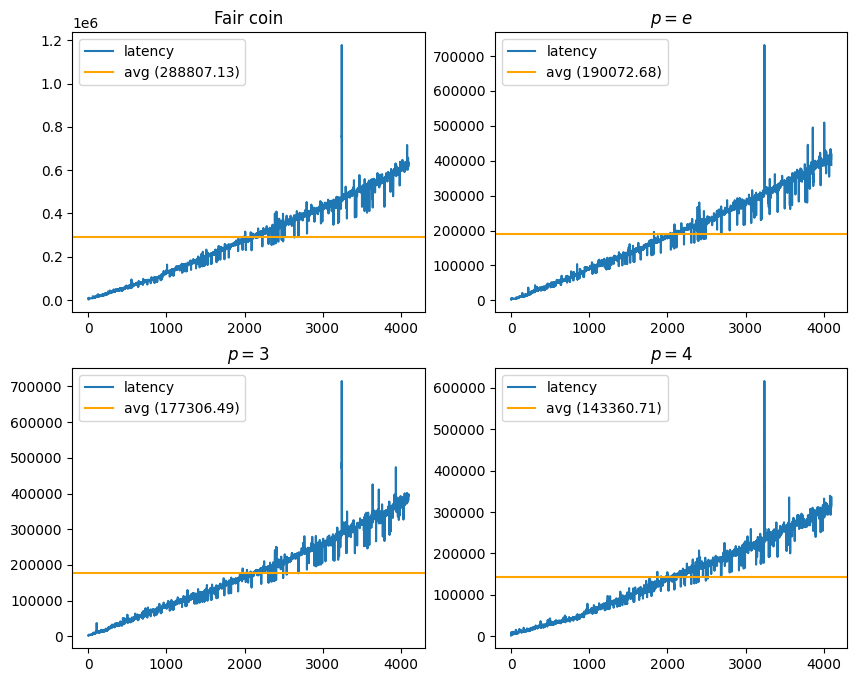
\includegraphics[height=0.42\textheight]{02-insert-latencies.png}
		\caption{Insert latency for different values of $p$}
		\label{fig:02-insert-latency}
	\end{center}
\end{figure}


\begin{figure}[H]
	\begin{center}
		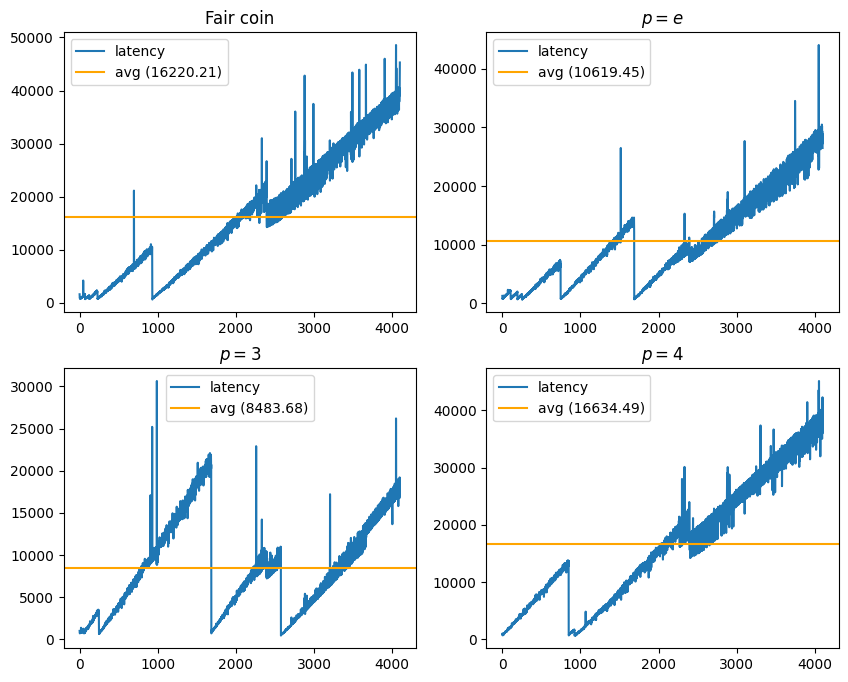
\includegraphics[height=0.42\textheight]{02-search-latencies}
		\caption{Search (get) latency for different values of $p$}
		\label{fig:02-search-latency}
	\end{center}
\end{figure}


\begin{figure}[H]
	\begin{center}
		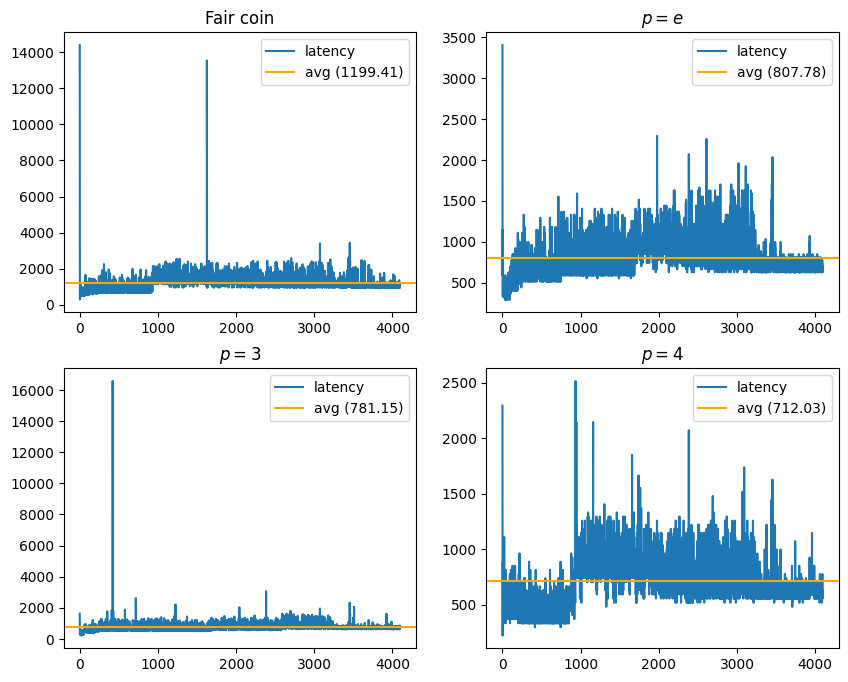
\includegraphics[height=0.42\textheight]{02-delete-latencies.png}
		\caption{Delete latency for different values of $p$}
		\label{fig:02-delete-latency}
	\end{center}
\end{figure}

